\documentclass[aspectratio=43]{beamer}
\usetheme{Boadilla}
\setbeamertemplate{navigation symbols}{}
\usepackage{graphicx} % Required for inserting images
\graphicspath{{./figures}}
\usepackage[autostyle=true]{csquotes}
\usepackage[T2A]{fontenc}
\usepackage[english, russian]{babel}
\usepackage{booktabs}
\usepackage{multirow}

\title{Interactive Speaker Recognition}
\subtitle{Применение обучения с подкреплением для решения задачи распознавания
          диктора}
\author[В.С.~Головин]{Головин Вячеслав Сергеевич \texorpdfstring{\newline}{, }
    {\small Шуранов Евгений Витальевич (руководитель)}}
\institute[ВШЭ]{Huawei CBG AI и ФКН ВШЭ СПб}
\date{07.06.2023}

\newcommand{\guesser}{\texttt{Guesser}}
\newcommand{\enquirer}{\texttt{Enquirer}}
\newcommand{\imgscale}{0.67}


\begin{document}

\frame{\titlepage}

\begin{frame}{Задача распознавания диктора (Speaker Recognition)}
    Два типа задач:
    \begin{enumerate}
        \item \textbf{Идентификация} --- по услышанной речи выбираем одного диктора из списка.
        \item \textbf{Верификация} --- по услышанной речи решаем, произнёс ли её конкретный диктор.
    \end{enumerate}\vspace{1em}

    Фактически обе задачи сводятся к определению меры похожести между двумя
    наборами данных:
    \begin{enumerate}
        \item Векторы признаков, вычисленные из полученных ранее аудиозаписей речи
        (\textbf{эмбеддинги дикторов} или голосовые подписи).\\
        \textit{Обозначение:} $G = {[g^k]}_{k=1}^K, \; K \in \mathbb{N}$.
        \item Векторы признаков аудиозаписей речи, полученных сейчас
        (\textbf{эмбеддинги} произнесенных \textbf{слов}).\\
        \textit{Обозначение:} $X = {[x^t]}_{t=1}^T, \; T \in \mathbb{N}$.
    \end{enumerate}
\end{frame}

\begin{frame}{Область исследования}
    \framesubtitle{Зачем нам \emph{Interactive} Speaker Recognition}
    Некоторые системы распознавания запрашивают y диктора произносимые фразы.
    Логично выбирать эти слова и фразы таким образом, чтобы
    \begin{itemize}
        \item точность распознавания была выше,
        \item количество запросов было меньше,
        \item они были разнообразными (боремся со спуфингом).
    \end{itemize}\vspace{1em}

    \textbf{Исследуемый подход:} использование нейросетевого RL-агента для
    выбора запрашиваемых слов.\vspace{1em}

    Подход предложен в статье \textit{A Machine of Few Words --- Interactive
    Speaker Recognition with Reinforcement Learning}, Mathieu Seurin et al.,
    INTERSPEECH 2020, arXiv:2008.03127v1.
\end{frame}

\begin{frame}{Цель и задачи}
    \textbf{Цель:} повышение точности систем распознавания диктора при помощи
    выбора запрашиваемых у диктора слов.\vspace{1em}

    \textbf{Задачи:}
    \begin{itemize}
        \item Воспроизведение результатов, достигнутых в исходной статье.
        \item Улучшение и модификация изначальной системы:
        \begin{itemize}
            \item Переход от идентификации к верификации.
            \item Использование произвольного набора запрашиваемых слов.
            \item Проверка работы при добавлении шума.
            \item Использование других эмбеддингов.
        \end{itemize}
    \end{itemize}
\end{frame}

\begin{frame}{Interactive Speaker Recognition}
    Здесь и далее изображения из \textit{A Machine of Few Words --- Interactive
    Speaker Recognition with Reinforcement Learning}, Mathieu Seurin et al.,
    INTERSPEECH 2020, arXiv:2008.03127v1.\vspace{1em}

    Использовался датасет TIMIT (630 дикторов, 20 слов).\vspace{1em}

    \begin{columns}

    \column{0.6\textwidth}
    \begin{figure}[bht]
        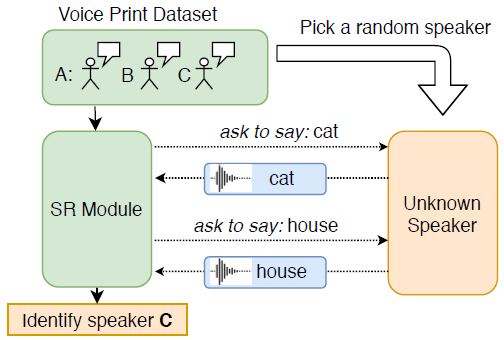
\includegraphics[width=.9\textwidth]{isr_game_large.png}
    \end{figure}

    \column{0.4\textwidth}
    Важные особенности статьи:
    \begin{enumerate}
        \item только идентификация
        \item фиксированный набор слов
        \item разные нейронные сети для запроса слов (\enquirer) и идентификации (\guesser)
    \end{enumerate}

    \end{columns}
\end{frame}

\begin{frame}{Архитектура \guesser}
\framesubtitle{Пытаемся угадать диктора}
    \begin{columns}
 
    \column{0.6\textwidth}
    \begin{figure}[bht]
    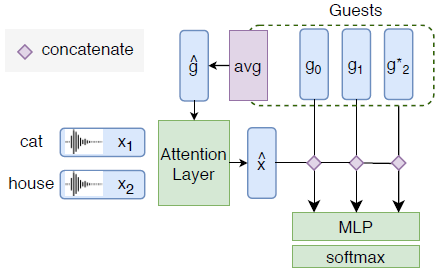
\includegraphics[width=.8\textwidth]{guesser.png}
    \end{figure}

    \column{0.4\textwidth}
    Входные данные:
    \begin{itemize}
        \item эмбеддинги дикторов\\
            $G = [g_1; g_2; \ldots g_K]$
        \item эмбеддинги слов\\
            $X = [x_1; x_2; \ldots x_T]$
    \end{itemize}
    Выходные данные:
    \begin{itemize}
        \item вероятности
            $\{P(g_i = g^*) \;|\; i=1..K\}$
    \end{itemize}
    \end{columns}

    \begin{block}{Обозначения}
    \begin{tabular}{l l}
        $K$ & количество гостей / дикторов\\
        $T$ & количество запрашиваемых слов
    \end{tabular}
    \end{block}
\end{frame}

\begin{frame}{Архитектура \enquirer}
\framesubtitle{Выбираем, какое слово мы спрашиваем у диктора}
    \begin{columns}

    \column{0.6\textwidth}
    \begin{figure}[bht]
    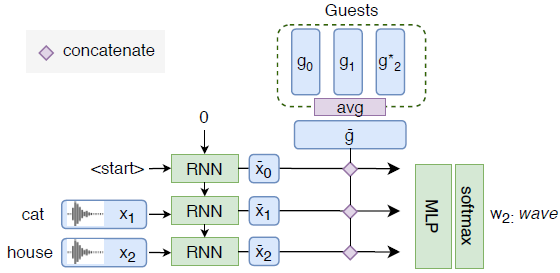
\includegraphics[width=.9\textwidth]{enquirer.png}
    % \caption{Архитектура блока Enquirer}
    \end{figure}

    \column{0.4\textwidth}
    Входные данные:
    \begin{itemize}
        \item среднее эмб. дикторов\\
            $\hat{g} = \frac{1}{K}{\sum_{i=1}^{K}{g_k}}$
        \item эмбеддинги слов\\
            $X = [x_1; x_2; \ldots; x_t]$
    \end{itemize}
    Выходные данные:
    \begin{itemize}
        \item вероятность выбрать каждое из слов
    \end{itemize}

    \end{columns}

    \begin{block}{Обозначения}
    \begin{tabular}{l l}
        $K$ & количество гостей / дикторов\\
        $T$ & количество запрашиваемых слов\\
        $t$ & количество запрошенных слов, $0 \leq t \leq T$
    \end{tabular}
    \end{block}
\end{frame}

\begin{frame}[t]{Обучение и тестирование \guesser{}}
    \framesubtitle{$K = 5$ дикторов  и $T = 3$ слова при обучении}
    \begin{columns}[T]
        \centering
        \column{.5\textwidth}
        \mbox{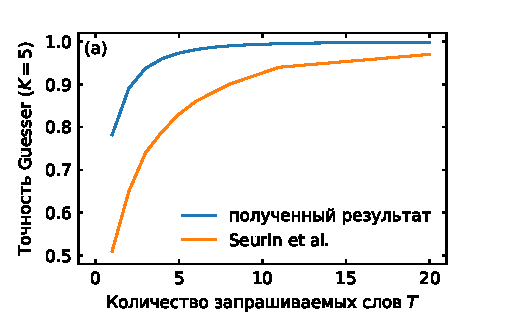
\includegraphics[scale=\imgscale]{../plots/old/word_sweep.pdf}}
        \column{.5\textwidth}
        \mbox{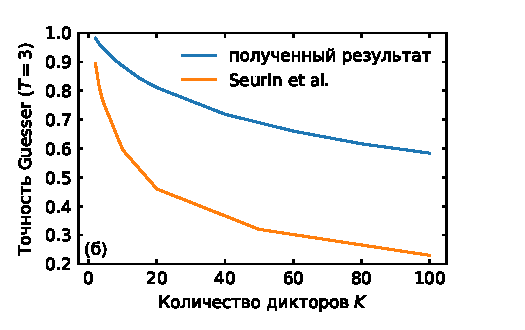
\includegraphics[scale=\imgscale]{../plots/old/guest_sweep.pdf}}
    \end{columns}\vspace*{1em}
    В качестве эмбеддингов использовались \textbf{x-vectors} из фреймворка
    \textbf{Kaldi}.\vspace{1em}

    Вероятно, главная причина расхождения результатов --- увеличение размерности
    эмбеддингов (512 вместо 128). Как и зачем в статье производилось понижение
    размерности неизвестно.
\end{frame}

\begin{frame}[t]{Обучение и тестирование \enquirer{}}
    \framesubtitle{$K = 5$ дикторов  и $T = 3$ слова при обучении}
    \begin{columns}[T]
        \centering
        \column{.5\textwidth}
        \mbox{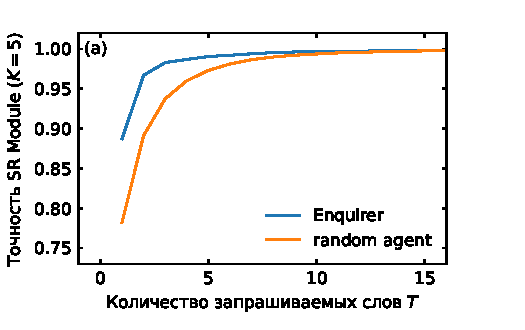
\includegraphics[scale=\imgscale]{../plots/old/word_sweep_enq.pdf}}
        \column{.5\textwidth}
        \mbox{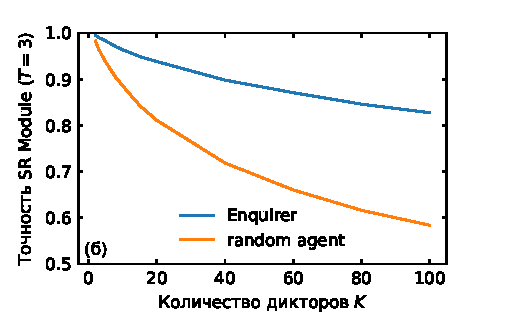
\includegraphics[scale=\imgscale]{../plots/old/guest_sweep_enq.pdf}}
    \end{columns}\vspace*{1em}

    Для обучения использовался \textbf{PPO}. Выбор слова при обучении и
    тестировании проводился по-разному:
    \begin{itemize}
        \item \texttt{train} --- сэмплирование из распределения,
        \item \texttt{test} --- $\arg \max$ по не использованным ранее словам.
    \end{itemize}\vspace{1em}

    Награда: $1.0$ --- \guesser{} угадал диктора, $0.0$ --- иначе.
\end{frame}

\begin{frame}[t]{\enquirer{} против эвристики}
    \framesubtitle{$K = 5$ дикторов  и $T = 3$ слова при обучении}
    \begin{columns}[T]
        \centering
        \column{.5\textwidth}
        \mbox{
            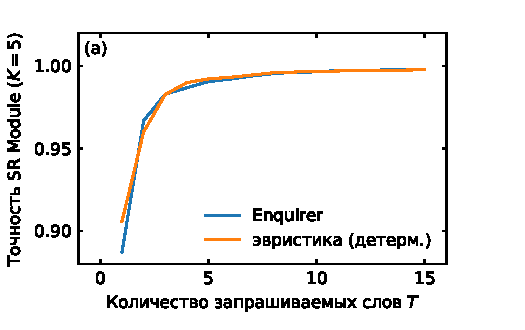
\includegraphics[scale=\imgscale]{../plots/old/word_sweep_heuristic.pdf}%
        }
        \column{.5\textwidth}
        \mbox{
            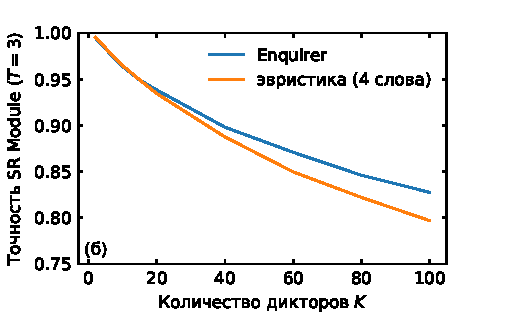
\includegraphics[scale=\imgscale]{../plots/old/guest_sweep_heuristic.pdf}
        }
    \end{columns}\vspace*{1em}

    Эвристический агент не обращает внимание на контекст и (практически) всегда
    запрашивает одни и те же слова.\vspace{1em}

    Для выбора слов используется средняя точность \guesser{} на валидационной
    выборке при использовании этого слова.
\end{frame}

\begin{frame}{От идентификации к верификации}
    \framesubtitle{$T = 3$ слова}
    \begin{center}
    \only<1>{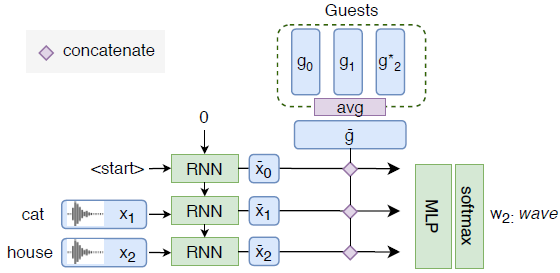
\includegraphics[scale=.6]{enquirer.png}}
    \only<2->{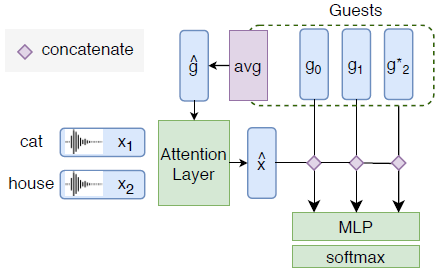
\includegraphics[scale=.6]{guesser.png}}
    \end{center}

    \begin{columns}
        \column{0.5\textwidth}
        \begin{itemize}
            \item<1-> \enquirer{}: не меняем ничего (даже веса)
            \item<2-> \guesser{}: меняем \texttt{softmax} на \texttt{sigmoid}
        \end{itemize}


        \column{0.5\textwidth}
        \onslide<3->{
        \begin{center}
            \begin{tabular}{c c}
                \toprule
                Выбор слов & Точность\\
                \midrule
                случайный & 0.895\\
                \enquirer{} & 0.933\\
                эвристика & 0.917\\
                \bottomrule
            \end{tabular}
        \end{center}
        }
        \end{columns}
\end{frame}


\begin{frame}{Другие эксперименты}
    \begin{enumerate}
        \item Подбор режима обучения.
        \begin{itemize}
            \item Для улучшения точности можно обучать модели в более тяжелых
            режимах (например, $K = 20$, $T = 2$).
        \end{itemize}
        \item \texttt{CodebookEnquirer} --- гибкая система выбора слов.
        \begin{itemize}
            \item Модифицируем \enquirer{} таким образом, что выбор осуществляется
            не из фиксированного набора слов, а из списка эмбеддингов.
            \item Работает (небольшое падение точности), даже если мы обучаем
            и тестируем модель на разных наборах слов.
        \end{itemize}

        \item Добавление шума
        \begin{itemize}
            \item Добавляем к аудиозаписям слов 6 видов шума из MUSAN\@.
            \item Не меняем тип шума в течение игры.
            \item Результаты принципиально не изменяются.
        \end{itemize}

        \item Альтернативные эмбеддинги
        \begin{itemize}
            \item Вместо \textbf{x-vector} используем нейронную сеть, обученную
            с помощью контрастного прогнозирующего кодирования (\textbf{CPC}).
            \item Существенное увеличение точности, \enquirer{} обучается.
        \end{itemize}
    \end{enumerate}
\end{frame}

\begin{frame}{Выводы}
    \begin{itemize}
        \item Исследованный подход работает --- точность идентификации 
        существенно повышается при добавлении выбирающего слова
        агента.
        \item Модель можно сделать практически полезной: легко перейти от
        идентификации к верификации и от фиксированного набора слов к
        произвольному.
        \item В большинстве режимов (очень) простая эвристика оказывается не хуже
        нейросетевого агента для выбора слов (\enquirer{}).
    \end{itemize}
\end{frame}

\begin{frame}[noframenumbering, plain]{}
    \centering
    \Huge
    Приложение
\end{frame}

\begin{frame}[noframenumbering, plain, fragile]{Псевдокод 1 итерации обучения
                                                \guesser{}}
\begin{lstlisting}[caption={Рассчёт функции потерь \guesser{}}]
speaker_ids = speakers.sample(size=K)
G = voice_prints.get(speaker_ids)
target = randrange(0, K)
word_inds = randrange(0, V, size=T)
X = word_vocab.get(speaker=speaker_ids[target],
                   words=word_inds)
probabilities = guesser.forward(G, X)
loss = cross_entropy(probabilities, target)
\end{lstlisting}
    \begin{block}{Обозначения}
    \begin{tabular}{l l}
        $K$ & количество гостей / дикторов\\
        $T$ & количество запрашиваемых слов\\
        $V$ & размер словаря --- число доступных для запроса слов
    \end{tabular}
    \end{block}
\end{frame}

\begin{frame}[noframenumbering, plain, fragile]{Псевдокод 1 эпизода ISR-игры}
\footnotesize
\begin{lstlisting}[caption={Интерактивная игра для обучения \enquirer{}}]
speaker_ids = speakers.sample(size=K)
G = voice_prints.get(speaker_ids)
target = randrange(0, K)

g_hat = G.mean(dim=0)
x_i = start_tensor
X = []
for i in range(T):
    probs = enquirer.forward(g_hat, x_i)
    if training:
        word_inds = multinomial(probs).sample()
    else:
        probs[previous_actions] = 0.0
        word_ind = argmax(probs)
    x_i = word_vocab.get(speaker=speaker_ids[target],
                         word=word_ind)
    X.append(x_i)

prediction = guesser.predict(G, X)
reward = 1 if prediction == target else 0
\end{lstlisting}
\end{frame}

\begin{frame}[noframenumbering, plain]{Результаты из статьи}
    \framesubtitle{$K = 5$ дикторов и $T = 3$ слова}
    \begin{columns}
        \centering
        \column{.5\textwidth}
        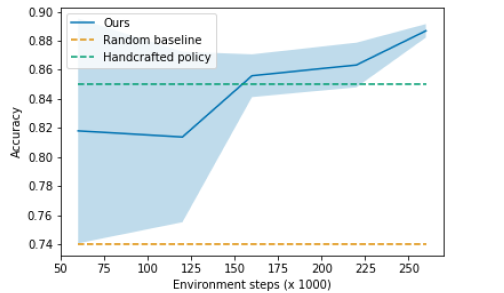
\includegraphics[scale=0.5]{isr_training.png}
        \column{.5\textwidth}
        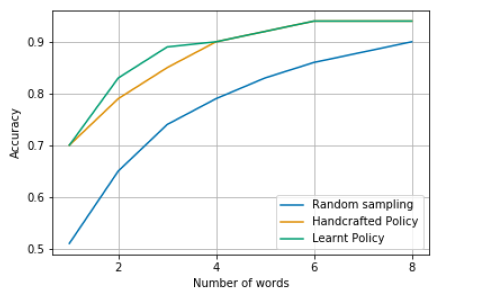
\includegraphics[scale=0.5]{isr_word_sweep.png}
    \end{columns}\vspace*{1em}

    RL-агент при выборе запрашиваемых слов учитывает контекст --- он опережает
    не только случайного агента, но и эвристического, выбирающего из
    подмножества ``лучших'' слов.\vspace*{1em}

    Преимущество RL-агента невелико и проявляется только при небольшом числе
    запрашиваемых слов.
\end{frame}

\begin{frame}[noframenumbering, plain]{Эвристический агент}
    \framesubtitle{Алгоритм работы}
    \begin{columns}[b]
        \column{.4\textwidth}
        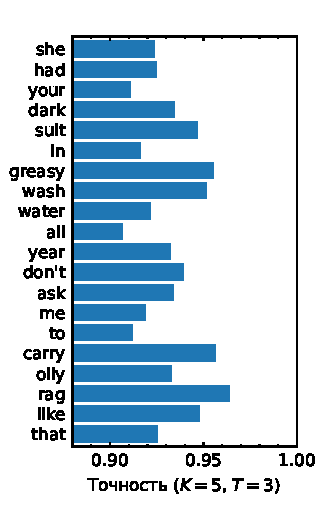
\includegraphics[height=.8\textheight]{../plots/word_scores.pdf}
        \column{.6\textwidth}
        \begin{enumerate}
            \item Рассчитываем точность на валидационной выборке.
            \item Сэмплируем из слов с самой высокой точностью.
        \end{enumerate}
        \begin{center}
            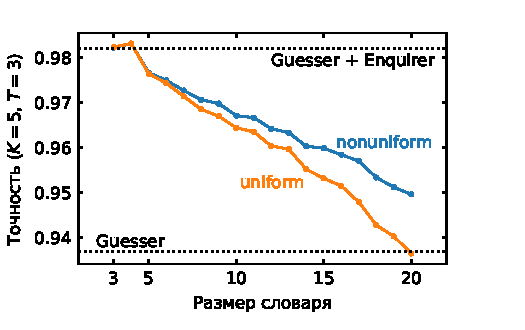
\includegraphics[scale=\imgscale]{../plots/heuristic.pdf}
        \end{center}
    \end{columns}
\end{frame}

\begin{frame}[noframenumbering, plain]{Обучение в более тяжелом режиме}
    \only<2>{
        \begin{table}[htb]
            \begin{tabular}{c c c}
                \toprule
                Выбор слов & Режим обучения & Точность\\
                \midrule
                случайный & \multirow{3}{4em}{$K = 5$\newline$T = 3$} & 0.937 \\
                \enquirer{} & & 0.982\\
                эвристика & & 0.984\\
                \midrule
                случайный & \multirow{3}{4em}{$K = 20$\\$T = 2$} & 0.951 \\
                \enquirer{} & & 0.989\\
                эвристика & & 0.988\\
                \bottomrule
            \end{tabular}
            \caption{Точность идентификации, $K = 5$ дикторов, $T = 3$
                     запрашиваемых слова}
        \end{table}
    }
    \only<1>{
        \begin{table}[htb]
            \begin{tabular}{c c c}
                \toprule
                Выбор слов & Режим обучения & Точность\\
                \midrule
                случайный & \multirow{3}{4em}{$T = 3$} & 0.895 \\
                \enquirer{} & & 0.933\\
                эвристика & & 0.917\\
                \midrule
                случайный & \multirow{3}{4em}{$T = 2$} & 0.913 \\
                \enquirer{} & & 0.947\\
                эвристика & & 0.945\\
                \bottomrule
            \end{tabular}
            \caption{Точность верификации, $T = 3$ запрашиваемых слова}
        \end{table}
    }
\end{frame}

\begin{frame}[noframenumbering, plain]{\texttt{CodebookEnquirer}}
    \framesubtitle{Мотивация и принцип работы}
    Очевидный недостаток архитектуры \enquirer{} --- строго фиксированный набор
    слов, при любом его изменении нужно обучать заново или делать fine-tuning.
    \vspace{1em}

    \begin{columns}

    \column{0.5\textwidth}
    \begin{figure}[bht]
    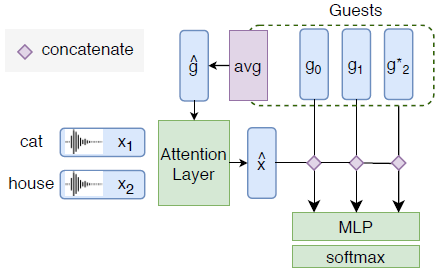
\includegraphics[width=\textwidth]{guesser.png}
    \end{figure}

    \column{0.5\textwidth}
    Предлагаемые изменения:
    \begin{itemize}
        \item MLP возвращает эмбеддинг слова, а не вероятности;
        \item добавляется \texttt{Codebook} --- набор (фиксированных)
            эмбеддингов слов;
        \item вероятность выбрать слово из \texttt{Codebook} обратно
            пропорциональна расстоянию между эмбеддингами.
    \end{itemize}

    \end{columns}
\end{frame}

\begin{frame}[noframenumbering, plain]{\texttt{CodebookEnquirer}}
    \framesubtitle{Результаты}
        \begin{table}[htb]
            \begin{tabular}{c c c}
                \toprule
                Выбор слов & Режим обучения & Точность\\
                \midrule
                случайный & \multirow{4}{4em}{$K = 5$\\$T = 3$} & 0.937 \\
                \enquirer{} & & 0.982 \\
                \texttt{CodebookEnquirer} & & 0.964\\
                \texttt{CodebookEnquirer} (половина слов) & & 0.970\\
                \midrule
                случайный & \multirow{4}{4em}{$K = 20$\\$T = 2$} & 0.951 \\
                \enquirer{} & & 0.989\\
                \texttt{CodebookEnquirer} & & 0.990\\
                \texttt{CodebookEnquirer} (половина слов) & & 0.980\\
                \bottomrule
            \end{tabular}
            \caption{Точность идентификации, $K = 5$ дикторов, $T = 3$
                     запрашиваемых слова}
        \end{table}
\end{frame}

\begin{frame}[noframenumbering, plain]{Добавление шума}
    \begin{itemize}
        \item 6 различных вариантов шума из датасета MUSAN для каждого слова:
        \texttt{rain}, \texttt{car}, \texttt{crowd}, \texttt{typing},
        \texttt{hum}, \texttt{white} --- а также исходная чистая аудиозапись.
        \item SNR 3~dB.
        \item Тип шума не меняется в течение эпизода.
    \end{itemize}

    \begin{table}[htb]
        \begin{tabular}{c c c}
            \toprule
            Модель & Идентификация & Верификация\\
            \midrule
            \guesser{} & 0.887 & 0.895\\
            \guesser{} + \enquirer{} & 0.946 & 0.934\\
            \guesser{} + эвристика (3 лучших) & 0.957 & 0.938\\
            \bottomrule
        \end{tabular}
        \caption{Точность идентификации и верификации в стандартных режимах
        ($T = 3$ слова, $K = 5$ гостей при идентификации)}
    \end{table}
\end{frame}
\end{document}